\chapter{An Exotic Spacetime: the Traversable Wormhole}
\label{app:xwormhole}

\emph{Nothing in this appendix describes \sgra.} It applies the simulator to
a hypothetical spacetime, the Double Negative (``Dneg'') wormhole designed for
the film \emph{Interstellar} by \citet{James2015wormhole} after the
traversable wormholes of \citet{MorrisThorne1988}. The point is to test the
code's generality: the same camera, sky and validation machinery, applied to a
metric that is not Kerr. In the simulator it is reached only through a
separate menu entry, \textsc{exotic (not sgr a*)}. A banner on screen says the
same, and none of its numbers enter any \sgra{} result.

\section{The metric and its rays}

The Dneg wormhole without gravity \citep[][eqs.~1 and 5]{James2015wormhole}
is
\begin{equation}
ds^2 = -dt^2 + d\ell^2 + r(\ell)^2\,(d\theta^2 + \sin^2\theta\,d\phi^2),
\label{eq:dneg}
\end{equation}
\begin{equation}
r(\ell) = \begin{cases}
\rho & |\ell| \le a, \\[2pt]
\rho + M\left[x \arctan x - \tfrac12 \ln(1 + x^2)\right],
\quad x = \dfrac{2(|\ell| - a)}{\pi M} & |\ell| > a .
\end{cases}
\end{equation}
The proper radial distance $\ell$ runs from $-\infty$ (the other universe)
through the cylindrical throat of radius $\rho$ and length $2a$ to $+\infty$
(our universe). The parameter $M$ sets how gently the mouths flare out.
\citet{James2015wormhole} describe the flare by the \emph{lensing width}
$W = 1.42953\,M$. It is the lateral distance in the embedding diagram over
which the surface turns from vertical to $45\degr$, which is where
$dr/d\ell = 1/\sqrt2$. Our code finds that point by bisection and reproduces
their coefficient: the numerical $W$ and the closed form agree to
$\XWhWdiff$. We use the film's wormhole throughout, as chosen by Christopher
Nolan \citep{James2015wormhole}: $2a = \XWhA\,\rho$ and $W = \XWhW\,\rho$
($M = \XWhM\,\rho$). The weak Newtonian potential that \citet{James2015wormhole}
added for the spacecraft's trajectory, $|\Phi| \lesssim 10^{-12}$, is
neglected for light, as in their own ray tracing.

With $p_t = -1$ the affine parameter is the time $t$. Two quantities are
conserved: $b = p_\phi$, and the total impact parameter $B^2 = p_\theta^2 +
b^2/\sin^2\theta$. The rays obey their equations (A.7):
\begin{equation}
\frac{d\ell}{dt} = p_\ell, \quad
\frac{d\theta}{dt} = \frac{p_\theta}{r^2}, \quad
\frac{d\phi}{dt} = \frac{b}{r^2\sin^2\theta}, \quad
\frac{dp_\ell}{dt} = B^2\,\frac{dr/d\ell}{r^3}, \quad
\frac{dp_\theta}{dt} = \frac{b^2\cos\theta}{r^2\sin^3\theta} .
\label{eq:dnegrays}
\end{equation}
The fp64 reference (\texttt{science/wormhole}) integrates
eq.~\eqref{eq:dnegrays} backward from the camera with an adaptive
Dormand--Prince scheme (tolerance $10^{-12}$). The camera uses their local
basis $e_x = e_{\hat\ell}$, $e_y = e_{\hat\phi}$, $e_z = -e_{\hat\theta}$. Along
every traced ray $|\Delta B^2|/B^2 \le \XWhMaxdB$ and the null condition
$|p_\ell^2 + B^2/r^2 - 1| \le \XWhMaxH$.

The live renderer uses the fact that, by spherical symmetry, each ray moves in
a plane through the centre (its lateral motion follows a great circle;
\citealp{James2015wormhole}). It therefore integrates the planar form
$d\ell/dt = p_\ell$, $d\psi/dt = B/r^2$, $dp_\ell/dt = B^2 r'/r^3$ in fp32 RK4.
Here $\psi$ is the angle swept from the camera's position, and the polar
singularity of eq.~\eqref{eq:dnegrays} never arises. Both integrations stop
once the ray is far out and receding ($|\ell| \ge 400\,\rho$ on the CPU,
$40\,\rho$ on the GPU). The remaining sweep, $\arcsin(B/r)$, is then added as
a straight line. Out there $dr/d\ell = 1 - O(M/\ell)$, so that completion errs
by $O(BM/\ell^2)$: moving the CPU stopping point from $400\,\rho$ to
$4000\,\rho$ shifts the Einstein rings below by at most
$\XWhRingShift$\,degrees.

\section{The edge of the other universe}

The radial equation has an exact first integral, $p_\ell^2 = 1 - B^2/r(\ell)^2$.
Since $r$ is smallest, $r = \rho$, along the whole throat, a ray gets through
if and only if $B < \rho$. A ray leaving the camera at angle $\alpha$ from the
direction of the wormhole has $B = r(\ell_c)\sin\alpha$. The other universe
therefore fills a disk on the camera's sky whose edge is exactly at
\begin{equation}
\sin\alpha_{\rm edge} = \rho / r(\ell_c),
\label{eq:dnegedge}
\end{equation}
whatever $a$ and $M$ are. This is our own elementary result; we use it as an
exact test of both tracers. Bisecting the CPU tracer for the edge reproduces
eq.~\eqref{eq:dnegedge} to $\XWhEdgeErr$\,degrees. The live GPU path is checked
on 2001-pixel strips along both image axes through the centre, using a
validation mask (rays that end in our universe are white, rays that end in the
other universe are black). All four edges (left, right, top, bottom) lie within
$\XWhGpuMaxPx$\,pixels of the CPU value at every camera distance
(Table~\ref{tab:xwormhole}).

Rays with $B$ just above $\rho$ wind around the throat before returning to our
universe, and they image our own sky many times in thin bands around the edge.
In every direction around the wormhole, exactly one of these rays ends at the
point of our celestial sphere directly behind the wormhole. Together they form
the \emph{Einstein ring}, the ring image of a source exactly behind the
wormhole \citep{James2015wormhole}. Its radius on the camera's sky is found by
bisecting for the ray whose final azimuth is $\phi_\infty = \pi$ (the camera
sits at $\phi = 0$).

\begin{table}
\centering
\caption{The Dneg wormhole of \emph{Interstellar} ($2a = \XWhA\,\rho$,
$W = \XWhW\,\rho$) seen from three distances: angular radius of the other
universe (CPU, equal to eq.~\ref{eq:dnegedge}) and of the Einstein ring. The
live GPU edges agree with the CPU edges within $\XWhGpuMaxPx$\,pixels in all
three cases.}
\label{tab:xwormhole}
\begin{tabular}{rrrr}
\toprule
$\ell_c/\rho$ & $r(\ell_c)/\rho$ & edge [deg] & Einstein ring [deg] \\
\midrule
15 & \XWhRFifteen & \XWhEdgeFifteen & \XWhRingFifteen \\
6 & \XWhRSix & \XWhEdgeSix & \XWhRingSix \\
2 & \XWhRTwo & \XWhEdgeTwo & \XWhRingTwo \\
\bottomrule
\end{tabular}
\end{table}

\section{The live demo}

The demo shows our universe as the Milky Way map of Chapter~\ref{ch:xspectral}.
For the other universe, whose sky nobody can know, it shows the same map turned
around with its colour channels swapped, so the dust lanes turn blue and it
cannot be mistaken for ours. This choice is illustrative only and is labelled
as such on screen. Dragging the mouse moves the camera around the wormhole, as
it does around \sgra, and the scroll wheel flies along $\ell$, through the
throat if you keep going. No colour shift is applied, because none exists:
$g_{tt} = -1$ everywhere, so a static camera receives light from either
universe at the frequency it was sent.
Figure~\ref{fig:xwormhole} shows the approach. The sine of the other
universe's angular radius grows as $1/r(\ell_c)$. Around its edge, inside the Einstein ring, lies the strongly
lensed image of our own Milky Way, with the Galactic Centre directly behind the
throat. This is the structure \citet{James2015wormhole} describe for the
film's wormhole. The far universe is seen through the mouth. The star field on
the camera's side forms secondary lensed images near the mouth's edge, which
are very thin for a wormhole this short. The Einstein ring lies just outside
the edge.

\begin{figure}
\centering
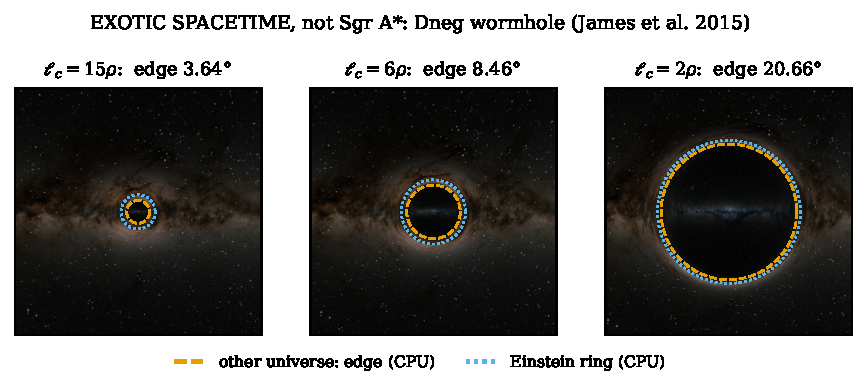
\includegraphics[width=\textwidth]{figures/fig_x_wormhole.pdf}
\caption{\emph{Not \sgra:} the Interstellar wormhole rendered live (GPU),
approached along $\ell$ (field of view 1.2\,rad). The fp64 CPU tracer's
results are overlaid: the edge of the other universe (dashed;
eq.~\ref{eq:dnegedge}) and the Einstein ring (dotted). Inside the edge is the
other universe (an illustrative recoloured sky); outside it is the lensed
Milky Way, with the Galactic Centre behind the throat.}
\label{fig:xwormhole}
\end{figure}
